\documentclass[border=5pt]{standalone}
\usepackage[T1]{fontenc}
\usepackage{lmodern}
\usepackage{pgfplots}
\usepgfplotslibrary{groupplots}
\pgfplotsset{compat=1.18}
\begin{document}
\sffamily
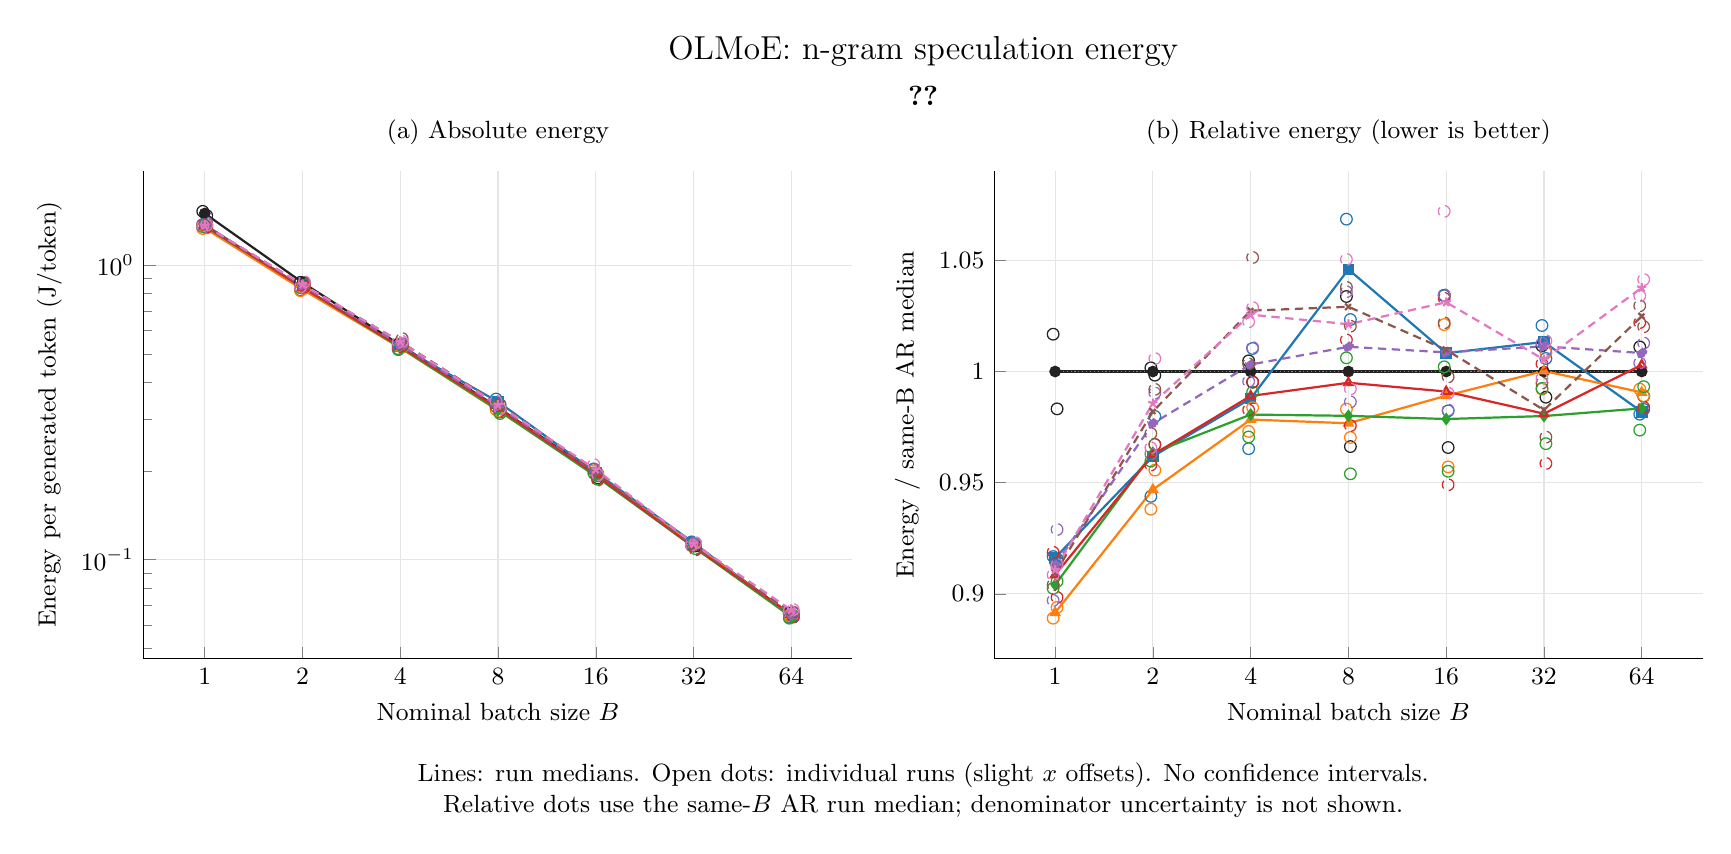
\begin{tikzpicture}
\definecolor{series0}{HTML}{222222}
\definecolor{series1}{HTML}{1f77b4}
\definecolor{series2}{HTML}{ff7f0e}
\definecolor{series3}{HTML}{2ca02c}
\definecolor{series4}{HTML}{d62728}
\definecolor{series5}{HTML}{9467bd}
\definecolor{series6}{HTML}{8c564b}
\definecolor{series7}{HTML}{e377c2}
\begin{groupplot}[group style={group size=2 by 1,horizontal sep=1.8cm},width=9.0cm,height=6.2cm,scale only axis,grid=major,grid style={gray!20},axis lines*=left,tick label style={font=\small},label style={font=\small},title style={font=\small},unbounded coords=jump]
\nextgroupplot[title={(a) Absolute energy},xlabel={Nominal batch size $B$},ylabel={Energy per generated token (J/token)},xtick={1,2,4,8,16,32,64},xticklabels={1,2,4,8,16,32,64},xmode=log,log basis x=2,minor x tick num=0,ymode=log,legend columns=8,legend to name=sharedlegend,legend style={draw=none,font=\small,/tikz/every even column/.append style={column sep=8pt}}]
\addplot+[color=series0,mark=*,mark size=1.7pt,mark options={fill=series0,draw=series0},line width=0.8pt] coordinates {(1,1.49822351074) (2,0.873144226074) (4,0.535546386719) (8,0.32869744873) (16,0.196280456543) (32,0.112606933594) (64,0.0650029296875)};
\addlegendentry{$\gamma=0$ (AR)}
\addplot+[only marks,forget plot,color=series0,mark=o,mark size=2.1pt,mark options={fill=white,line width=0.45pt}] coordinates {(0.986097544263,1.52337487793) (1.01409845894,1.47307214355) (1.97219508853,0.874584838867) (2.02819691788,0.871703613281) (3.94439017705,0.538112670898) (4.05639383575,0.532980102539) (7.8887803541,0.339786865234) (8.11278767151,0.317608032227) (15.7775607082,0.202987182617) (16.225575343,0.189573730469) (31.5551214164,0.113905761719) (32.451150686,0.111308105469) (63.1102428328,0.0657220458984) (64.9023013721,0.0642838134766)};
\addplot+[color=series1,mark=square*,mark size=1.7pt,mark options={fill=series1,draw=series1},line width=0.8pt] coordinates {(1,1.37276409912) (2,0.83982824707) (4,0.529030883789) (8,0.343795654297) (16,0.197904663086) (32,0.11410333252) (64,0.0638260498047)};
\addlegendentry{$\gamma=1$}
\addplot+[only marks,forget plot,color=series1,mark=o,mark size=2.1pt,mark options={fill=white,line width=0.45pt}] coordinates {(0.986097544263,1.37358544922) (1.01409845894,1.37194274902) (1.97219508853,0.824145141602) (2.02819691788,0.855511352539) (3.94439017705,0.516973388672) (4.05639383575,0.541088378906) (7.8887803541,0.351213867187) (8.11278767151,0.336377441406) (15.7775607082,0.203001342773) (16.225575343,0.192807983398) (31.5551214164,0.114938232422) (32.451150686,0.113268432617) (63.1102428328,0.0637552490234) (64.9023013721,0.0638968505859)};
\addplot+[color=series2,mark=triangle*,mark size=1.7pt,mark options={fill=series2,draw=series2},line width=0.8pt] coordinates {(1,1.3357199707) (2,0.826771728516) (4,0.523986877441) (8,0.321049438477) (16,0.194145935059) (32,0.112635803223) (64,0.0643924560547)};
\addlegendentry{$\gamma=2$}
\addplot+[only marks,forget plot,color=series2,mark=o,mark size=2.1pt,mark options={fill=white,line width=0.45pt}] coordinates {(0.986097544263,1.33207470703) (1.01409845894,1.33936523437) (1.97219508853,0.81910168457) (2.02819691788,0.834441772461) (3.94439017705,0.521122680664) (4.05639383575,0.526851074219) (7.8887803541,0.323146118164) (8.11278767151,0.318952758789) (15.7775607082,0.200425537109) (16.225575343,0.187866333008) (31.5551214164,0.111718383789) (32.451150686,0.113553222656) (63.1102428328,0.0644892578125) (64.9023013721,0.0642956542969)};
\addplot+[color=series3,mark=diamond*,mark size=1.7pt,mark options={fill=series3,draw=series3},line width=0.8pt] coordinates {(1,1.35453063965) (2,0.841231628418) (4,0.525182434082) (8,0.322149475098) (16,0.192088439941) (32,0.110353149414) (64,0.0639254760742)};
\addlegendentry{$\gamma=3$}
\addplot+[only marks,forget plot,color=series3,mark=o,mark size=2.1pt,mark options={fill=white,line width=0.45pt}] coordinates {(0.986097544263,1.35214306641) (1.01409845894,1.35691821289) (1.97219508853,0.837967163086) (2.02819691788,0.84449609375) (3.94439017705,0.519783691406) (4.05639383575,0.530581176758) (7.8887803541,0.330718994141) (8.11278767151,0.313579956055) (15.7775607082,0.196696655273) (16.225575343,0.187480224609) (31.5551214164,0.111751464844) (32.451150686,0.108954833984) (63.1102428328,0.063291015625) (64.9023013721,0.0645599365234)};
\addplot+[color=series4,mark=triangle,mark size=1.7pt,mark options={fill=series4,draw=series4},line width=0.8pt] coordinates {(1,1.36125299072) (2,0.840465209961) (4,0.529667541504) (8,0.327036499023) (16,0.194515930176) (32,0.110472167969) (64,0.0651954956055)};
\addlegendentry{$\gamma=4$}
\addplot+[only marks,forget plot,color=series4,mark=o,mark size=2.1pt,mark options={fill=white,line width=0.45pt}] coordinates {(0.986097544263,1.37645129395) (1.01409845894,1.3460546875) (1.97219508853,0.836453369141) (2.02819691788,0.844477050781) (3.94439017705,0.526285400391) (4.05639383575,0.533049682617) (7.8887803541,0.333372802734) (8.11278767151,0.320700195312) (15.7775607082,0.202743652344) (16.225575343,0.186288208008) (31.5551214164,0.112991821289) (32.451150686,0.107952514648) (63.1102428328,0.0664340820312) (64.9023013721,0.0639569091797)};
\addplot+[color=series5,mark=pentagon*,mark size=1.7pt,mark options={fill=series5,draw=series5},line width=0.8pt] coordinates {(1,1.36788793945) (2,0.852762878418) (4,0.537238342285) (8,0.332349914551) (16,0.197972045898) (32,0.113881347656) (64,0.0655438842773)};
\addlegendentry{$\gamma=5$}
\addplot+[only marks,forget plot,color=series5,mark=o,mark size=2.1pt,mark options={fill=white,line width=0.45pt}] coordinates {(0.986097544263,1.34399829102) (1.01409845894,1.39177758789) (1.97219508853,0.840803710937) (2.02819691788,0.864722045898) (3.94439017705,0.533150268555) (4.05639383575,0.541326416016) (7.8887803541,0.340489379883) (8.11278767151,0.324210449219) (15.7775607082,0.203061645508) (16.225575343,0.192882446289) (31.5551214164,0.114026611328) (32.451150686,0.113736083984) (63.1102428328,0.0652528076172) (64.9023013721,0.0658349609375)};
\addplot+[color=series6,mark=x,mark size=1.7pt,mark options={fill=series6,draw=series6},line width=0.8pt] coordinates {(1,1.36236297607) (2,0.857458129883) (4,0.550198425293) (8,0.338269287109) (16,0.198198425293) (32,0.110657043457) (64,0.0666187133789)};
\addlegendentry{$\gamma=6$}
\addplot+[only marks,forget plot,color=series6,mark=o,mark size=2.1pt,mark options={fill=white,line width=0.45pt}] coordinates {(0.986097544263,1.3545670166) (1.01409845894,1.37015893555) (1.97219508853,0.848781860352) (2.02819691788,0.866134399414) (3.94439017705,0.537389282227) (4.05639383575,0.563007568359) (7.8887803541,0.341136962891) (8.11278767151,0.335401611328) (15.7775607082,0.200582397461) (16.225575343,0.195814453125) (31.5551214164,0.112026611328) (32.451150686,0.109287475586) (63.1102428328,0.0669243164063) (64.9023013721,0.0663131103516)};
\addplot+[color=series7,mark=star,mark size=1.7pt,mark options={fill=series7,draw=series7},line width=0.8pt] coordinates {(1,1.36468310547) (2,0.860706054688) (4,0.549237976074) (8,0.335692626953) (16,0.20239239502) (32,0.113211303711) (64,0.0674515991211)};
\addlegendentry{$\gamma=7$}
\addplot+[only marks,forget plot,color=series7,mark=o,mark size=2.1pt,mark options={fill=white,line width=0.45pt}] coordinates {(0.986097544263,1.36118737793) (1.01409845894,1.36817883301) (1.97219508853,0.843213623047) (2.02819691788,0.878198486328) (3.94439017705,0.547535888672) (4.05639383575,0.550940063477) (7.8887803541,0.345262695312) (8.11278767151,0.326122558594) (15.7775607082,0.210414916992) (16.225575343,0.194369873047) (31.5551214164,0.112260131836) (32.451150686,0.114162475586) (63.1102428328,0.0672116699219) (64.9023013721,0.0676915283203)};
\nextgroupplot[title={(b) Relative energy (lower is better)},xlabel={Nominal batch size $B$},ylabel={Energy / same-B AR median},xtick={1,2,4,8,16,32,64},xticklabels={1,2,4,8,16,32,64},xmode=log,log basis x=2,minor x tick num=0,scaled y ticks=false,yticklabel style={/pgf/number format/fixed,/pgf/number format/precision=2}]
\addplot+[color=series0,mark=*,mark size=1.7pt,mark options={fill=series0,draw=series0},line width=0.8pt] coordinates {(1,1) (2,1) (4,1) (8,1) (16,1) (32,1) (64,1)};
\addplot+[only marks,forget plot,color=series0,mark=o,mark size=2.1pt,mark options={fill=white,line width=0.45pt}] coordinates {(0.986097544263,1.01678745995) (1.01409845894,0.983212540047) (1.97219508853,1.0016499139) (2.02819691788,0.998350086103) (3.94439017705,1.00479189897) (4.05639383575,0.995208101029) (7.8887803541,1.0337374584) (8.11278767151,0.966262541596) (15.7775607082,1.03416909759) (16.225575343,0.965830902412) (31.5551214164,1.01153417541) (32.451150686,0.988465824585) (63.1102428328,1.0110628277) (64.9023013721,0.988937172303)};
\addplot+[color=series1,mark=square*,mark size=1.7pt,mark options={fill=series1,draw=series1},line width=0.8pt] coordinates {(1,0.916261218222) (2,0.961843670256) (4,0.987833914874) (8,1.04593344312) (16,1.00827492748) (32,1.01328869261) (64,0.981894971681)};
\addplot+[only marks,forget plot,color=series1,mark=o,mark size=2.1pt,mark options={fill=white,line width=0.45pt}] coordinates {(0.986097544263,0.91680943422) (1.01409845894,0.915713002223) (1.97219508853,0.943882026578) (2.02819691788,0.979805313935) (3.94439017705,0.965319534391) (4.05639383575,1.01034829536) (7.8887803541,1.06850195687) (8.11278767151,1.02336492938) (15.7775607082,1.03424124005) (16.225575343,0.982308614899) (31.5551214164,1.02070297764) (32.451150686,1.00587440757) (63.1102428328,0.980805777985) (64.9023013721,0.982984165377)};
\addplot+[color=series2,mark=triangle*,mark size=1.7pt,mark options={fill=series2,draw=series2},line width=0.8pt] coordinates {(1,0.891535849709) (2,0.946890220225) (4,0.978415484514) (8,0.976732371111) (16,0.989125145101) (32,1.00025637523) (64,0.990608521251)};
\addplot+[only marks,forget plot,color=series2,mark=o,mark size=2.1pt,mark options={fill=white,line width=0.45pt}] coordinates {(0.986097544263,0.889102792394) (1.01409845894,0.893968907023) (1.97219508853,0.938105825029) (2.02819691788,0.955674615421) (3.94439017705,0.973067307684) (4.05639383575,0.983763661345) (7.8887803541,0.983111123655) (8.11278767151,0.970353618566) (15.7775607082,1.02111815226) (16.225575343,0.957132137945) (31.5551214164,0.992109279808) (32.451150686,1.00840347066) (63.1102428328,0.992097711942) (64.9023013721,0.989119330559)};
\addplot+[color=series3,mark=diamond*,mark size=1.7pt,mark options={fill=series3,draw=series3},line width=0.8pt] coordinates {(1,0.904091165261) (2,0.963450943494) (4,0.980647889905) (8,0.980079025079) (16,0.978642720343) (32,0.979985387154) (64,0.983424537656)};
\addplot+[only marks,forget plot,color=series3,mark=o,mark size=2.1pt,mark options={fill=white,line width=0.45pt}] coordinates {(0.986097544263,0.902497562421) (1.01409845894,0.905684768101) (1.97219508853,0.959712196522) (2.02819691788,0.967189690467) (3.94439017705,0.970567077468) (4.05639383575,0.990728702342) (7.8887803541,1.00615017068) (8.11278767151,0.954007879483) (15.7775607082,1.00212042879) (16.225575343,0.955165011899) (31.5551214164,0.992403054388) (32.451150686,0.967567719919) (63.1102428328,0.973664047594) (64.9023013721,0.993185027718)};
\addplot+[color=series4,mark=triangle,mark size=1.7pt,mark options={fill=series4,draw=series4},line width=0.8pt] coordinates {(1,0.908578046575) (2,0.962573175041) (4,0.989022715192) (8,0.994946873748) (16,0.991010177996) (32,0.98104232522) (64,1.00296241906)};
\addplot+[only marks,forget plot,color=series4,mark=o,mark size=2.1pt,mark options={fill=white,line width=0.45pt}] coordinates {(0.986097544263,0.918722262784) (1.01409845894,0.898433830366) (1.97219508853,0.957978469263) (2.02819691788,0.967167880819) (3.94439017705,0.982707405824) (4.05639383575,0.995338024561) (7.8887803541,1.01422388285) (8.11278767151,0.975669864646) (15.7775607082,1.03292837155) (16.225575343,0.949091984443) (31.5551214164,1.0034179751) (32.451150686,0.958666675339) (63.1102428328,1.02201673602) (64.9023013721,0.983908102099)};
\addplot+[color=series5,mark=pentagon*,mark size=1.7pt,mark options={fill=series5,draw=series5},line width=0.8pt] coordinates {(1,0.913006590569) (2,0.976657524556) (4,1.00315930722) (8,1.01111193845) (16,1.00861822611) (32,1.01131736761) (64,1.00832200321)};
\addplot+[only marks,forget plot,color=series5,mark=o,mark size=2.1pt,mark options={fill=white,line width=0.45pt}] coordinates {(0.986097544263,0.897061273821) (1.01409845894,0.928951907317) (1.97219508853,0.962960855525) (2.02819691788,0.990354193586) (3.94439017705,0.995525843842) (4.05639383575,1.0107927706) (7.8887803541,1.03587472674) (8.11278767151,0.986349150171) (15.7775607082,1.03454846745) (16.225575343,0.982687984766) (31.5551214164,1.01260737407) (32.451150686,1.01002736115) (63.1102428328,1.00384410258) (64.9023013721,1.01279990385)};
\addplot+[color=series6,mark=x,mark size=1.7pt,mark options={fill=series6,draw=series6},line width=0.8pt] coordinates {(1,0.909318914238) (2,0.982034931088) (4,1.02735904664) (8,1.02912051315) (16,1.0097715727) (32,0.982684102351) (64,1.02485709028)};
\addplot+[only marks,forget plot,color=series6,mark=o,mark size=2.1pt,mark options={fill=white,line width=0.45pt}] coordinates {(0.986097544263,0.904115445319) (1.01409845894,0.914522383158) (1.97219508853,0.972098119652) (2.02819691788,0.991971742525) (3.94439017705,1.00344115011) (4.05639383575,1.05127694318) (7.8887803541,1.03784487591) (8.11278767151,1.02039615039) (15.7775607082,1.02191731665) (16.225575343,0.997625828744) (31.5551214164,0.994846478391) (32.451150686,0.97052172631) (63.1102428328,1.02955846341) (64.9023013721,1.02015571714)};
\addplot+[color=series7,mark=star,mark size=1.7pt,mark options={fill=series7,draw=series7},line width=0.8pt] coordinates {(1,0.9108675012) (2,0.985754734424) (4,1.02556564603) (8,1.02128151055) (16,1.03113880304) (32,1.0053670773) (64,1.03767013957)};
\addplot+[only marks,forget plot,color=series7,mark=o,mark size=2.1pt,mark options={fill=white,line width=0.45pt}] coordinates {(0.986097544263,0.908534252847) (1.01409845894,0.913200749553) (1.97219508853,0.965720894517) (2.02819691788,1.00578857433) (3.94439017705,1.02238742012) (4.05639383575,1.02874387194) (7.8887803541,1.05039663875) (8.11278767151,0.992166382347) (15.7775607082,1.07201155275) (16.225575343,0.990266053331) (31.5551214164,0.99692024508) (32.451150686,1.01381390952) (63.1102428328,1.03397908748) (64.9023013721,1.04136119165)};
\addplot[forget plot,gray,densely dotted,domain=1:64] {1};
\end{groupplot}
\path (group c1r1.north west) -- node[above=1.2cm,font=\large] {OLMoE: n-gram speculation energy} (group c2r1.north east);
\path (group c1r1.north west) -- node[above=0.7cm] {\ref{sharedlegend}} (group c2r1.north east);
\path (group c1r1.south west) -- node[below=1.2cm,align=center,font=\small] {Lines: run medians. Open dots: individual runs (slight $x$ offsets). No confidence intervals.\\Relative dots use the same-$B$ AR run median; denominator uncertainty is not shown.} (group c2r1.south east);
\end{tikzpicture}
\end{document}
